\mychapter{2}{Opis riešenia}

%\centerline{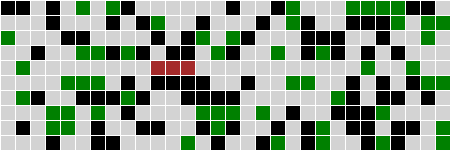
\includegraphics[width=0.4\textwidth]{images/cervik}}


%klucove slova ... špecifikovať, analyzovať , poukázať, predstaviť, vytvoriť, rozobereať, načrtnúť
\section{Špecifikácia požiadaviek}
V nasledujúcej sekcii opíšeme základný model fungovania aplikácie, analyzujeme  požiadavky a naznačíme spôsob jej realizácie. Pre lepšie pochopenie aplikácie si pomôžeme jednoduchým príkladom procesu, na ktorom vyniknú hlavné výhody nášho systému. V rámci nášho systému sa špecialne zameriame na model riadenia systému pomocou rolí.  

\subsection{Základný opis aplikácie}
Zistili sme, že Workflow management systému je silný nástroj, ktorý umožní používateľovi oddeliť a jasne znázorniť procesnú časť od aplikácie. Tento systém ponúka mnohé výhody. Jednou z možností ako WfMS implementovať je použitím Petriho sietí. Petriho siete sú jasne formálne definované a matematicky overené. Ako základ pre fungovanie našej aplikácie sme sa preto rozhodli použiť práve Petriho siete. Pri aplikácii Petriho siete na WfMS prechody predstavujú úlohy, ktoré za sebou nasledujú v určitom poradí. Tieto úlohy môžeme rôzne definovať.  Príklad takejto úlohy je napríklad vypísanie daňového priznania, schválenie žiadosti alebo iné. V našej aplikácii bude ku každému prechodu v sieti možné priradiť formulár, ktorý pokryje vačšinu bežných požiadaviek. Pre vypísanie daňového priznania sa teda bude dať jednoducho vypísať formulár, ktorý bude obsahovať potrebné políčka ako krátka odpoveď, dlhá odpoveď, zaškrtávacie políčka prípadne výber z viacerých možností. Každú úlohu musí niekto spustiť a vykonať. Je treba teda definovať prístup riadenia v aplikácii. Pre tieto účely sme zvolili systém riadenia za pomoci rolí, ktorý sa ukázal ako flexibilné riešenie našich požiadaviek. Ku každému prechodu v procese bude okrem furmuláru pridelená rola ktorá môže daný prechod spustiť. 

Naznačili sme spôsob vytvávarania bussines procesov prostredníctvom Petriho sietí. Aby však daná aplikácia mohla fungovať ako plnohodnotné WfMS potrebujeme aplikačné rozhranie, ktoré bude nad vytvoreným procesom zabezpečovať jeho správne fungovanie. Naša aplikácia bude poskytovať webové rozhranie, ktoré umožní užívateľom používať náš systém bez nutnosti sťahovať dodatočný softvér. Takisto sa tým vyhneme problémom spojených s kompatibilitou odlišných operačných systémov.  Na strane servera budeme využívať kombináciu jazyka PHP s databázovým systémom MySQL. Na strane klienta využijeme framework  Jquery, ktorý je rýchly a nenáročný na pamäť.

Kľúčovou výhodou WfMS je možnosť oddeliť proces od aplikačnej časti. Veľa firiem používa rovnaké alebo veľmi podobné procesy. Predstavme si dve rôzne pekárne. V zjednodušenom pohľade môžeme povedať, že pre obidve pekárne platí rovnaký proces výroby chleba. Jediné v čom sa tieto pekárne odlišujú je zamestnanecká štruktúra. Náš systém by umožnil obidvom pekárňam použiť rovnaký proces. Ak je možné propoužiť rovnaké procesy pre viacero firiem, vzniká tu možnosť procesy predávať. V našej aplikácii je preto dôležitou súčasťou portál, ktorý okrem poskytnutia tvorby procesov a jeho následného používania, poskytne možnosť vyhľadávať a prepoužívať procesy, ktoré už boli vytvorené.  


\subsection{Funkcia rolí v aplikácii}
V biznis procesoch vačšinu úloh vykonávajú fyzické osoby. V každej firme je niekoľko zamestnancov, ktorí majú rôzne právomoci.Zároveň však môžeme vidieť ich neustálu fluktuáciu. Zamestnanci do firmy prichádzajú a aj odchádzajú. Takisto sa stáva, že zamestnanec zmení pozíciu vo firme a dostane tak nové právomoci. Pre management riadenia takéhoto systému nám nestačí využitie klasických modelov, prípadne systém na správu takéhoto systému by bol vysoko nákladný. Z týchto dôvodou vačšina workflow management systémou využíva model systému prístupu na základe rolí RBAC. Pre potreby našej aplikácie preto využijeme základy tohoto modelu. V každom procese priradíme rolu na samotný proces, aby sme vedeli určiť, kto môže spustiť nový prípad. Zároveň v petriho sieti definujeme ku každému prechodu jednu rolu, ktorá môže daný prechod spustiť. Samotnéprávomoci danej role nad prechodom sú dané určené vo dátovej časti.Vo formulári ku prechodu sa dajú políčka nastaviť ako povinné, upraviteľné a viditeľné. To nám zabezpečí ekvivalent k právomociam read, write. 

\subsection{Referencie}
Role v procese zabezpečia prenos prístupových práv z úloh na užívateľa. V rámci jednej role si môžeme predstaviť skupinu užívateľov, ktorí majú určité spoločné prístupové práva vo firme. V niektorých procesoch však treba zabezpečiť, aby dve od seba závislé úlohy, mohol spustiť len ten samý užívateľ. Samotné role túto funkcionalitu nedokážu zabezpečiť . V našej aplikácii je nutné ju explicitne zadefinovať. Do našej aplikácie sme použili systém referencii na prechody v Petriho sieti. Do nášho projektu sme implementovali dva typy referencii : referencia na prechod a referencia na prvého užívateľa z role. 

Najskôr opíšeme referenciu na prechod. Referencia na prechod zabezpečí, aby ten samý užívateľ ktorý spustí prechod, na ktorý odkazuje referencia, bol jediný oprávnený na spustenie prechodu s touto referenciou. Jednoduchým príkladom je ak rozložíme jeden zložitý prechod , ktorý musí vykonať ten samý užívateľ na dve menšie. Predstavme si napríklad podpísanie tlačiva. Ku tlačivu treba podpísať aj jeho kópiu. Náš prvý prechod predstavuje podpísanie tlačiva a druhý prechod je priradený k podpísaniu kópie tlačiva. Podpísanie kópie obsahuje v sebe referenciu na prvý prechod s podpísaním originálnehotlačiva. V praxi to znamená, že obidve tlačivá musí podpísať tá istá osoba. 


V procese však môžu existovať úlohy, ktoré sa v určitom prípade nikdy nevykonajú. Príkladom v Petriho sieti je podmienené vykonanie prechodov na základe OR-splitu. V prípade, že by sme namodelovali proces s referenciu na takýto prechod, pri vykonávaní procesu by sme sa dostali do stavu, kedy by nikto daný prechod nemohol spustiť a tým pádom by nebolo možné proces ukončiť. Takýto stav by bol nežiadúci a spôsobil by mnoho problémov. Druhým problémom ktorý vzniká je, že v procese vopred nevieme určiť poradie vykonávania jednotlivých úloh. Chceme aby prechod1 aj prechod2 spustil rovnaký človek z role. Nevieme však v akom poradí budú prechody za sebou nasledovať. Z týchto dôvodov sme sa rozhodli pridať "referenciu na prvého užívateľa z role". Táto referencia rieši obidva problémy zároveň. Prechod, ktorý bude označený touto referenciou , bude môcť spustiť jedine užívateľ, ktorý v procese prvýkrát spustil prechod pod takou rolou akú má proces s referenciou. V prípade, že taká neexistuje, znamená to, že dosiaľ nebol spustený žiaden prechod, ktorý by obsahoval danú rolu. V tomto prípade bude môcť prechod spustiť ktorýkoľvek užívateľ, ktorý je priradený k danej role. Jednou z alternatívnych riešení bolo vytvoriť zásobník referencii ...

%teraz mi napadlo, že by bolo dobré to spraviť tak, že by bola napr. referencia1 - priradená prechodom 2,3,4 a ktokoľvek by prvý spustil hociktorý z týchto prechodov by následne určil danú referenciu. Je to taká modifikácia nášho prvý z role. Ale umožňovalo by to mať viacero referencii tej samer role v jednom procese a zjednodušilo by to systém , pretože by to fungovalo rovnako dobre aj na náš prvý prípad "referencia na prechod" 


%ked vyhladavam užívateľov, nemal by som dať limit... aj ked to mi neotestujú :D
\subsection{Určenie požiadaviek}
Aplikačným výstupom tejto bakalárskej práce je web stránka, ktorej účelom je vytvoriť jednoduché a intuitívne aplikačné rozhranie pre priraďovanie užívateľov k roliam. V aplikácii by sa mali dať vyhľadať všetci užívateľia vo firme. Pre rýchlejšie vyhľadávanie a prehľadné údaje bude možné užívateľov zotriediť do kategórie podľa rolí. Užívatelia, ktorí nemajú priradenú žiadnu rolu, budú mať vlastnú podsekciu. Vďaka tomu bude mať firma každého užívateľa pod kontrolou, aby mal priradelenú minimálne jednu rolu. Užívatelia sa budú dať zoradiť podľa ich id, mena, priezviska alebo e-mailovej adresy. V každej podsekcii umožníme vyhľadávať konkrétneho užívateľa na základe vstupu . Tento vstup sa porovná s id,menom, priezviskom aj emailom každého užívateľa z vybranej podsekcie. Niektoré firmy majú vo svojej štruktúre niekoľko desiatok zamestnancov.   Každý užívateľ sa bude dať jednotne aj skupinovo priradiť k požadovanej role. Zároveň bude možné osobitne spravovať role pre konkrétneho člena firmy. Ďalšou funkcionalitou aplikácie je management rolí vo firme. Do firmy bude možné vložiť nové role, prípadne niektoré role odstrániť. Pri odstránení role z firmy, treba dať pozor, aby sme nemohli odstrániť role ktoré firma práve používa na vykonávanie vlastných procesov. Takýmto spôsobom bude možné do firmy pridať role z xml súboru vygenerované v aplikácii na vytváranie a prideľovanie rolí k procesom od Kristiána Stroku. Túto funkcionalitu bude možné pri integrácii plne odstrániť. Zároveň má aplikácia poskytovať rozhranie, prostredníctvom ktorého  bude možné výstup od Kristiána Stroku možné uložiť do databázy. 

\section{Návrh}
V nasledujúcej kapitole podrobne opíšeme fungovanie celého systému, pričom sa bližšie zameriame na konkrétnu imolementáciu a v krátkosti vysvetlíme jednotlivé časti systému, tak ako sme si ich rozdelili. Na začiatku na obrázku popíšeme model celého systému. Následne sa pozrieme na príklad systému , ktorý bude možné za pomoci našej aplikácie vytvoriť. V rámci tohto príkladu za pomoci ilustrácii a opisu bližšie rozoberieme jednotlivé časti celej aplikácie. Na konci si ukážeme možné scénare a životné cykly.......
	
	\subsection{Model fungovania aplikácie}
		%\begin{figure}
		%	\centering
		%	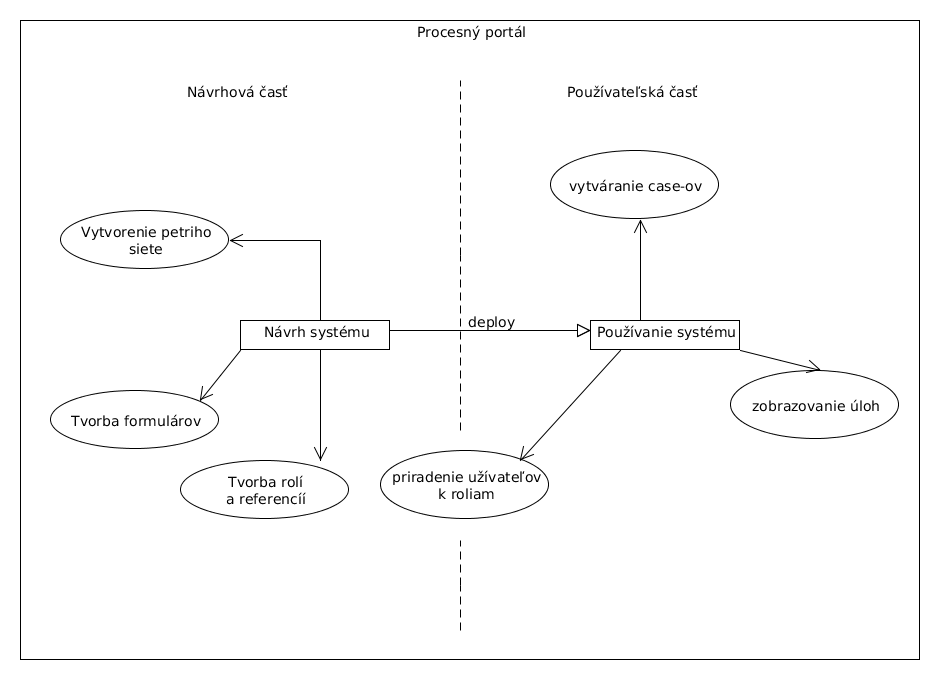
\includegraphics[width=0.7\linewidth]{../../uml/model_apk}
		%	\caption{}
		%	\label{fig:model_apk}
		%\end{figure}
		
	\subsubsection{Schvaľovanie bakalárskych prác}
	Pre bližšie porozumenie fungovania aplikácie si ukážeme príklad schvaľovania bakalárskej práce. Najprv si definujeme celý proces vrátane osôb ktoré sa daného procesu zúčastňujú. Následne si ukážeme príklad na vytvorenie procesu a jeho spracovanie v aplikácii. Celý proces ilustrujeme obrázkami 
	----TODO---
	
	Najprv si celý proces predstavíme z pohľadu -----TODO----- . Na stránke úvodnej stránke sa zaregistrujeme a prihlásime. Vytvoríme si firmu .... . 
		
	
	\subsection{Životný cyklus}
	

\section{Implementácia}
V tejto časti sa zameriame podrobný opis implementácie modulu na správu a priraďovanie rolí k užívateľom. Podrobne si vysvetlíme fungovanie rolí v systéme, vysvetlíme databázový model a popíšeme celkovú architektúru a spôsob implementácie rolí v našom systéme. Rozoberieme možné bezpečnostné riziká a spôsob ich riešenia.

	\subsection{Popis architektúry}
	Základnou myšlienkou RBAC architektúry je odstrániť priame priraďovanie práv k užívateľom. Tento výsledok sa zabezpečí pridaním medzikroku a teda rolí medzi samotných užívateľov a ich právomocii .Samotná implementácia tejto architektúry závisí od konkrétneho systému a jeho architektúry. Naša aplikácia sa zameriava na vytvorenie WfMS za pomoci Petriho sietí. Ako prvé si definujeme základnú architektúru. Na Obr. \ref{fig:model_rbac_v_aplikacii} môžeme zreteľne vidieť dve nezávislé časti fungovania workflow systému. V ľavej časti ilustácie vidíme sekciu, ktorá sa zaoberá  prideľovaním  užívateľou k roliam, zatiaľ čo pravá časť znázorňuje proces samotný. Vo firme je vďaka tomu zabezpečené, aby sa procesy mohli vytvárať nezávisle od užívateľov. Priraďovanie práv je zabezpečené väzbou medzi rolami a procesmi. Pre správnu funkcionalitu je však potrebné, aby firma mala priradené tie role, ktoré sú použité v jednotlivých procesoch, ktoré firma využíva. Definovanie prístupových práv je zabezbečené nad samotnými prechodmi v sieti.
	
	\begin{figure}[h]
		\centering
		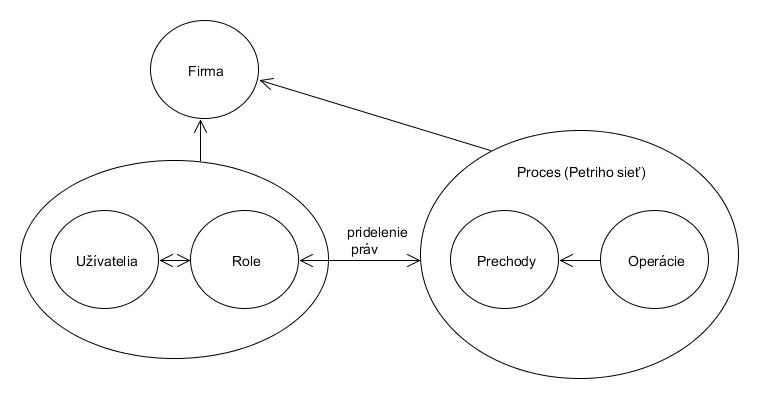
\includegraphics[width=0.9\linewidth]{images/roles_in_petri_model}
		\caption{ Model RBAC v aplikácii}
		\label{fig:model_rbac_v_aplikacii}
	\end{figure}
	
	\subsubsection{Priraďovanie užívateľou k roliam}
	V našej aplikácii nechceme aby bol užívateľ viazaný len na jednu firmu. Chceme aby pod rovnakým účtom mohol figurovať vo viacerých firmách, prípadne mal možnosť si založiť vlastnú. Preto je potrebné, aby sa užívatelia neviazali len na samotnú rolu. V aplikácii bude väzba užívateľa na rolu závislá od konkrétnej firmy. V každej firme bude môcť administrátor, užívateľ s právami na riadenie rolí, mať možnosť priradiť užívateľa ku konkrétnej role, ktorá je vo firme obsiahnutá. Samotný užívateľ môže byť tým pádom priradený vo viacerých firmách, pričom v každej firme bude mať iné práva. Na obrázku  \ref{fig:user_to_roles} môžeme vidieť zjednodušený model mapovania právomocí užívateľa prostredníctvom systému rolí.
	Šedé pozadie v roli znamená, že užívateľ je k roli priradený.  V rovnakom procese vidíme, že užívateľ, ktorý môže vo firme 1 spustiť prechod 1 , nie je oprávnený vykonať prechod 1 aj vo firme 2, pretože v nej nemá priradenú rolu. Vo firme 2 môže spustiť iba prechod 2.
	
		\begin{figure}[h]
			\centering
			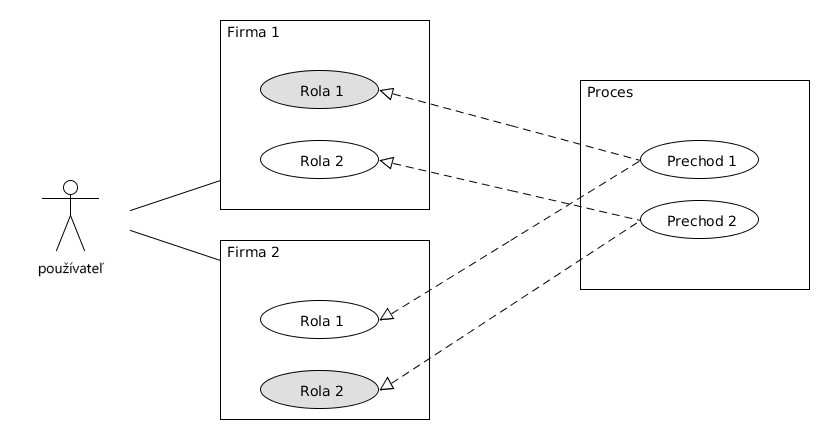
\includegraphics[width=0.9\linewidth]{images/user_to_roles}
			\caption{ Model RBAC v aplikácii}
			\label{fig:user_to_roles}
		\end{figure}
	
	
	\subsubsection{Riadenie právomocí}	
	Zadefinovali sme si ako sa v aplikácii mapujú užívatelia na role. V nasledujúcej časti si bližšie definujeme pravidlá pre spúšťanie prechodov v sieti, rovnako ako aj samotné právomoci ktoré daná rola v procese nadobudne. 
	
	V kapitole \ref{kap:teoria_petriho_siete_na_workflow} sme zistili, že Petriho sieť musí obsahovať dva špeciálne prechody (začiatočný a konečný) aby mohla spĺnať požiadavky na vykonávanie funkcie Workflow management systému. Začiatočný stav je dôležitý aby bolo možné určiť začiatok 

	V procese je jasne definované, ktorá rola môže vytvoriť nový prípad, pričom ku každému prechodu je pridelená práve jedna rola . Ak chce firma takýto proces používať,  musí mat tieto role  obsiahnuté vo svojej organizačnej štruktúre. Je preto potrebné, aby zakaždým , čo firma preberie proces na používanie, sa do firmy pridali tie role, ktoré sú v procese obsiahnuté. 	
	
		\begin{figure}[h]
			\centering
			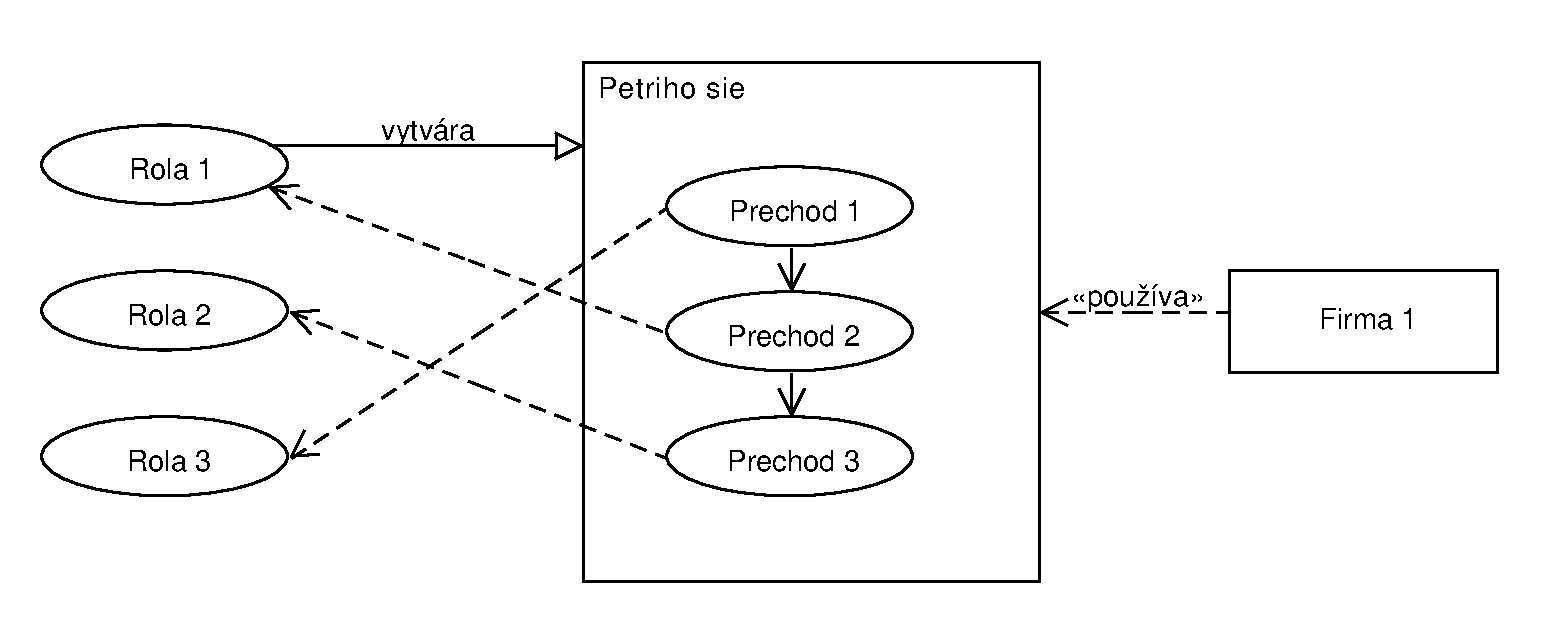
\includegraphics[width=0.9\linewidth]{images/roles_permissions}
			\caption{ Model RBAC v aplikácii}
			\label{fig:roles_permissions}
		\end{figure}		
	
	
	\subsection{Databázový model}
	TODO
	\subsection{Grafický model}
	TODO

\section{Overenie riešenia}
TODO
	

